\PassOptionsToPackage{table}{xcolor}
\documentclass{article}
\usepackage[colorlinks]{hyperref}
\usepackage[margin=1.25in]{geometry}
\usepackage{amsmath,amssymb,amsthm,booktabs,tikz}
\usepackage[final]{microtype}
\usepackage{libertine}
\usepackage[varqu]{zi4}
\usepackage[libertine]{newtxmath}
\usepackage[T1]{fontenc}
\usepackage[utf8]{inputenc}
\usepackage{tabto}


\newcommand{\ENT}[1]{\textcolor{colA}{\textbf{#1}}}
\newcommand{\AT}[1]{\textcolor{colB}{\textit{#1}}}
\newcommand{\RS}[1]{\textcolor{colC}{\textsc{#1}}}
\newcommand{\CON}[1]{\textcolor{colG}{\texttt{#1}}}
\newcommand{\IR}[1]{\textcolor{black!50}{\sout{#1}}}

\usepackage[normalem]{ulem}
\newcommand{\key}[1]{\underline{\smash{#1}}}
\newcommand{\pkey}[1]{\dashuline{\smash{#1}}}

\newcommand{\ent}[1]{\textbf{#1}}
\newcommand{\attr}[1]{\emph{#1}}
\newcommand{\rel}[1]{\textsf{#1}}
\newcommand{\domain}[1]{(of type \textsc{#1})}

%% Tikz
\usepackage{tikz}
\usetikzlibrary{arrows.meta,calc,decorations.pathreplacing,shapes.geometric,overlay-beamer-styles}
\tikzset{
    >=Stealth,
    er/.style={
        attr/.append style={align=center,draw,thick,ellipse,text width=2cm,text height=1.5ex,text depth=.25ex,font=\strut},
        entity/.append style={align=center,draw,thick,rectangle,text width=2cm,text height=2ex,text depth=.25ex,minimum height=1cm,font=\strut},
        rel/.append style={align=center,draw,thick,diamond,text width=2cm,text height=1.5ex,text depth=.25ex,font=\strut,fill=black!10,scale=0.65},
        isa/.append style={regular polygon, regular polygon sides=3,draw,thick,scale=0.65,font={ISA}},
        total/.append style={ultra thick},
        weak/.append style={ultra thick},
        once/.append style={->},
        strict/.append style={-Arc Barb[]},
        every edge/.append style={draw,thick}
    }
}



% Seven colors safe for use color blindness.
% Colors taken from doi:10.1038/nmeth.1618. 
\definecolor{colA}{RGB}{230,159,0}
\definecolor{colB}{RGB}{86,180,233}
\definecolor{colC}{RGB}{0,158,115}
\definecolor{colD}{RGB}{240,228,66}
\definecolor{colE}{RGB}{0,114,178}
\definecolor{colF}{RGB}{213,94,0}
\definecolor{colG}{RGB}{204,121,167}


%% Metadata
\author{Jelle Hellings}
\date{
    3DB3: Databases -- Fall 2021\\[0.5cm]
    Department of Computing and Software\\
    McMaster University
}

\begin{document}
\title{Explanation and Model Solution for\\``Assignment 1: The Entity-Relationship Model''}
\maketitle

\section*{Foreword}

This document consists of three parts. First, we have annotated the original assignment \emph{description} to highlight all information of interest. This part constitutes the main analysis step that should precede the design of the ER-diagram and the writing of the report. Second, we have included the \emph{ER-Diagram} based on our analysis. Finally, we have given a \emph{short report} describing the ER-Diagram, highlighting our choices, and describing all constraints that could not be included in the diagram.

\section*{Analysis}

In the analysis, we use the following text annotations:
\begin{center}
\begin{tabular}{lp{12cm}}
\ENT{an entity}&The highlighted piece of text resembled an entity-like object.\\
\AT{an attribute}& The highlighted piece of text resembled an attribute of some entity-like object.\\
\RS{a relationship}& The highlighted piece of text resembled a relationship between entity-like objects.\\
\CON{a constraint}& The highlighted piece of text resembled a constraint on data.\\
\IR{not-relevant}&The highlighted piece of text is not relevant (e.g., context, application details, ...)\\
\end{tabular}
\end{center}

\IR{A local chain of cinemas has decided that their current information system is not sufficient in a modern world in which online ticket sales are the norm. As the first step to renew their system, the owner of the cinema approached a consultant firm that drafted requirements for the new information system. Following is the high-level description of these requirements.}

\IR{First, the system will store information about several cinemas.} Each \ENT{cinema} has a \CON{unique} \AT{name} and an \AT{address}.\footnote{An entity cinema with attributes name and address. We can use name as the primary key.} In the past, cinema names have changed (e.g., due to renovations and grant reopenings).\footnote{Names can change. Non-changing unique identifiers are often easier to work with. Hence, we can opt for a numeric automatically-generated identifier.} \RS{Per cinema, the system will also maintain information per room}. Each \ENT{room} has a \CON{unique} \AT{number} \CON{within the cinema} \IR{(e.g., smaller cinemas have Room one to Room five)}.\footnote{The entity cinema owns rooms. Hence, room is a weak entity, there is an identifying relationship to cinema, and the room number can be a partial key.} Per \ENT{room}, the system can keep track of the \AT{characteristics of the cinema installation}.\footnote{The simplest solution here is to have an attribute for each basic room characteristic.} These characteristics include
\begin{enumerate}
\item the \AT{\emph{screen type}} (e.g., normal, purpose-built IMAX, digital IMAX) and \AT{\emph{screen size}};
\item the \AT{\emph{projector type}} (e.g., analog or digital, resolutions, supported 3D modes,  48FPS, and so on);
\item the \AT{\emph{sound system}} (e.g., the number of speakers and the supported sound options such Dolby Atmos, Dolby Digital, and DTS); and
\item the \AT{\emph{available accessibility options}}.\footnote{This is under-specified. This could be a simple Boolean option (e.g., a flag that is true when the room is designed with accessibility in mind) or this could be a whole range of features (e.g., special seating, elevator access, ramp access, \dots). Without further information, it is impossible to determine what the owner exactly wants. For now, we can choose for the simple Boolean option.}
\end{enumerate}
\IR{This information is not only available for cinema visitors, but will also be communicated to private parties that are looking to hire a room (e.g., for a corporate event). Finally, per room the system also needs to know the exact seat arrangement, as the online system will allow customers to order tickets for specific seats}. Hence, the system keeps track, \RS{per} \ENT{room}, of each \ENT{seat} and---per seat---its \AT{location} in the room, the \AT{row} it is in, and the \AT{seat number} (within the row).\footnote{The entity room owns seats and seats are uniquely identified within a room by its row and seat number. Hence, seat is a weak entity, there is an identifying relationship to room, and the row and seat number can be the partial key. }\textsuperscript{,}\footnote{It is unclear what location exactly is. In many cinemas, seat locations are purely determined by row and number. It is possible, however, that the cinema uses a per-room coordinate for each seat so that the seating arrangement can be visualized in any ticket ordering tools. This needs clarification from the cinema owner! For now, we keep location as an attribute.} Furthermore, some seats are standard \AT{reserved} for disabled people.\footnote{We can make this a Boolean attribute of each seat.}

\IR{Second, the system needs to store information for each screening.} Each \ENT{screening} is \RS{assigned a single room} and \AT{timeslot} and the system distinguishes between \CON{three types of screenings}\footnote{We can represent a screening as an entity that has a timeslot (a begin-time followed by an end-time) and an exact-one-to-many relationship to its assigned room. We will use a unique identifier for each screening, as no clear identifier is provided in the text. As there are three types of screenings, we can consider using an ISA hierarchy if the three types behave differently.}\textsuperscript{,}\footnote{We note that practically speaking, the combination of rooms and timeslot should be unique (we do not want double booked rooms). Unfortunately, making combinations of rooms and timeslots unique does not eliminate double booked rooms: E.g., the timeslots (October 1, 5pm--7pm) and (October 1, 6pm--8pm) \emph{are} unique values from a data perspective, but also overlap in practice.}: \ENT{normal screenings} will \RS{show a \CON{single} film} \IR{and will be offered via normal ticket prices}; \ENT{special screenings} can \RS{show \CON{one-or-more} films} \IR{with a special ticket price, e.g., a marathon with a higher ticket price or a classic film at a reduced ticket price}; and \ENT{private screenings} \IR{(as part of hired rooms)}.\footnote{There are clear distinctions between the three types of screenings: normal screenings have exactly one film associated to them, special screenings have one-or-more films associated with them, and private screenings do not have films associated with them. Hence,\ENT{screening} is an ISA hierarchy. We note that the screening types do not overlap and each \ENT{screening} should be a specializations.} \IR{For each \ENT{public screening}, the system keeps track which films are shown.}\footnote{This is redundant information: we already know how public screenings (normal and special screenings) keep track of films.} \IR{This film information is provided by the film distributors in a standard format: for now, the system represents this external information via an} entity \ENT{Film} with an \AT{attribute \CON{\key{fid}}}.\footnote{Exact description of an entity Film with one primary key attribute fid.} \IR{If a screening will show multiple films (as part of special screening), then each of these films will be shown in the same room and the ticket of the customer assign the same seat during each film.}

\IR{Finally, and most importantly, the system will support} sales and reservations. Via an (online) sale, customers can buy one or more \RS{tickets} for a specific \ENT{screening} and that are assigned a \ENT{seat} on sale. \IR{Customers that do not feel comfortable with paying online} can reserve their seats online \IR{and buy a ticket for these reservations at the counter (these reservations will be cancelled 45 minutes before the start of the film)}.\footnote{There are two types of ticket orders: one can buy or reserve a ticket for a screening. Either will allocate a specific seat for that screening. We represent both orders via a relationship between screenings and seats. To assure we can distinguish between sales and reservations, we maintain a Boolean attribute paid.} For each sale, we keep track of \AT{how} they are made (online, ticket machine, at the counter) and whether the sale was related to a \AT{reservation}.\footnote{How becomes a standard attribute. Furthermore, we keep track of whether this order was originally a reservation. Note that non-reservations must always be paid (as they are direct sales)!} \IR{The cinema chain owners plan to analyze this data to see what factors influence the willingness of customers to buy and reserve tickets via their online system.} Furthermore, we keep track of the \AT{paid price} \IR{(which can depend on coupons, special actions, payment method, or room and film options)}.\footnote{The paid price will become a final attribute.}\textsuperscript{,}\footnote{There is an important hidden constraint here: if a screening  is in room $X$, a seat is in room $Y$, and there exists an order for this combination of screening and seat, then $X = Y$ (they must refer to the same room).}\textsuperscript{,}\footnote{The ticket sale description contains a lot of application and process logic (e.g., reservations are cancelled 45 minutes before the start of the film) and relatively little detail on what \emph{exactly} needs to happen with all the data. E.g., it is unspecified whether the system needs to keep track of all reservations (including those cancelled) separately from the sales. We have chosen for a minimal method that can store all information requested, but not more.}

\paragraph{Notes on the analysis}

The analysis already revealed all elements that are relevant for the ER-Diagram. Furthermore, the footnotes discuss the main choices we can make, that we did make, and what open questions are still around. These footnotes will serve as a direct basis for the report (and, in practice, will be starting points with further meetings with the cinema owners to figure out all requirements).

From the analysis, we have seen that the description is not very precise in the following areas:
\begin{itemize}
\item room characteristics (especially accessibility options);
\item seat locations; and
\item the sale infrastructure.
\end{itemize}
For all these, we have chosen \emph{simple} solutions that can store the mentioned information. In practice, I expect these areas to be the main topics for future iterations on the requirements with the cinema owners.

\section*{Model Solution}
We have derived an ER-Diagram that can represent all information present in the description. The resultant ER-Diagram can be found in Figure~\ref{fig:er}. Next, we provide a high-level overview of the ER-Diagram, discuss the choices made, and present all constraints.

Each cinema is represented by an entity \ent{Cinema} with attributes \attr{name} \domain{text} and \attr{address} \domain{text}. Names are unique and can change. As names can change, the \attr{name} be tricky to use as primary keys. Hence, we assigned cinemas numeric automatically-generated identifiers \attr{cid} \domain{integer}.

Cinemas own rooms that are identified within their cinema by a room number. Hence, we model \ent{Room} as a weak entity with an identifying relationship \rel{In\_Cinema} to \ent{Cinema} and with a partial key \attr{room\_number} \domain{integer}. Rooms have characteristics. From the description it is unclear to what level of details these characteristics need to be stored, but the examples provided for screen type, screen size, projector type, and sound system indicate that these characteristics can be stored in simple attributes of the weak entity \ent{Room} Hence, we add attributes \attr{screen\_type} \domain{text}, \attr{screen\_size} \domain{integer}, \attr{projector\_type} \domain{text}, and \attr{sound\_system} \domain{text}. For the accessibility options we have chosen to add an attribute \attr{access\_flag} \domain{Boolean} that represents a flag that is set to true when the room is designed with accessibility in mind.

Rooms have seats and seats are uniquely identified within a room by its row and seat number. Hence, we model \ent{Seat} as a weak entity with an identifying relationship \rel{In\_Room} to \ent{Room} and with a partial key \attr{row} \domain{integer} and \attr{number} \domain{integer}. It is unclear whether the row and number of a seat already specify its location. Hence, we have added a placeholder attribute \attr{location} \domain{text} to \ent{Seat} to keep track of the per-room coordinate of that seat. Finally, we added an attribute \attr{reserved\_flag} \domain{Boolean} to \ent{Seat} that indicates whether this seat is reserved for disabled people.

We represent each screening by an entity \ent{Screening}, we introduce an automatically-generated identifier \attr{sid} as no clear identifier is provided in the text, and we represent the timeslot by two attributes \attr{begin\_time} \domain{timestamp} and \attr{end\_time} \domain{timestamp}. We assign each screening to exactly one room via the relationship \rel{Scr\_Room}. There are three types of screenings and there are clear distinctions between them: normal screenings have exactly one film associated to them, special screenings have one-or-more films associated with them, and private screenings do not have films associated with them. Hence, we introduce an ISA-hierarchy with root \ent{Screening} and specializations \ent{NormalS}, \ent{PrivateS}, and \ent{SpecialS}. We represent films by an entity \ent{Film} with primary key \attr{fid} \domain{integer}, we associate exactly-one film to each normal screening via the relationship \rel{NS\_Shows} between \ent{NormalS} and \ent{Film}, and we associate one-or-more films to each special screening via the relationship \rel{SS\_Shows} between \ent{SpecialS} and \ent{Film}.

We have chosen for a minimal method that can store all the described information for sales and reservations: we represent \emph{all} sales and reservations via the relationship \rel{Ticket\_Order} between entities \ent{Screening} and \ent{Seat}. To assure we can distinguish between sales and reservations, \rel{Ticket\_Order} has an attribute \attr{paid\_flag} \domain{Boolean} that is true when the ticket is already paid (a sale). Furthermore, we keep track of whether this order was originally a reservation via the attribute \attr{reserved\_flag} \domain{Boolean}. Finally, we keep track of how the order was made via attribute \attr{how} \domain{text} and what the price of the order is via attribute \attr{price} \domain{decimal}.

The following constraints are not expressed in the ER-Diagram:
\begin{itemize}
\item The attribute \attr{name} of entity \ent{Cinema} is unique.
\item In entity \ent{Screening}, values for the attribute \attr{begin\_time}  must be after values for the attribute \attr{end\_time}.
\item In relationship \rel{Ticket\_Order}, the attribute \attr{paid\_flag} must be true if the attribute \attr{reserved\_flag} is false (if a ticket is not reserved, it must be a sale order).
\item If an \ent{screening} $S_1$ is assigned to room $X$ and a \ent{seat} $S_2$ is in room $Y$, and there exists a \rel{Ticket\_Order} between $S_1$ and $S_2$, then the rooms $X$ and $Y$ must be the same room.
\item Timeslots for entities \ent{Screening} that are assigned to the same room should not overlap.
\item The screening types do not overlap and each \ent{Screening} must be a specializations.
\end{itemize}


\begin{figure}
    \centering
    \makebox[0pt]{
    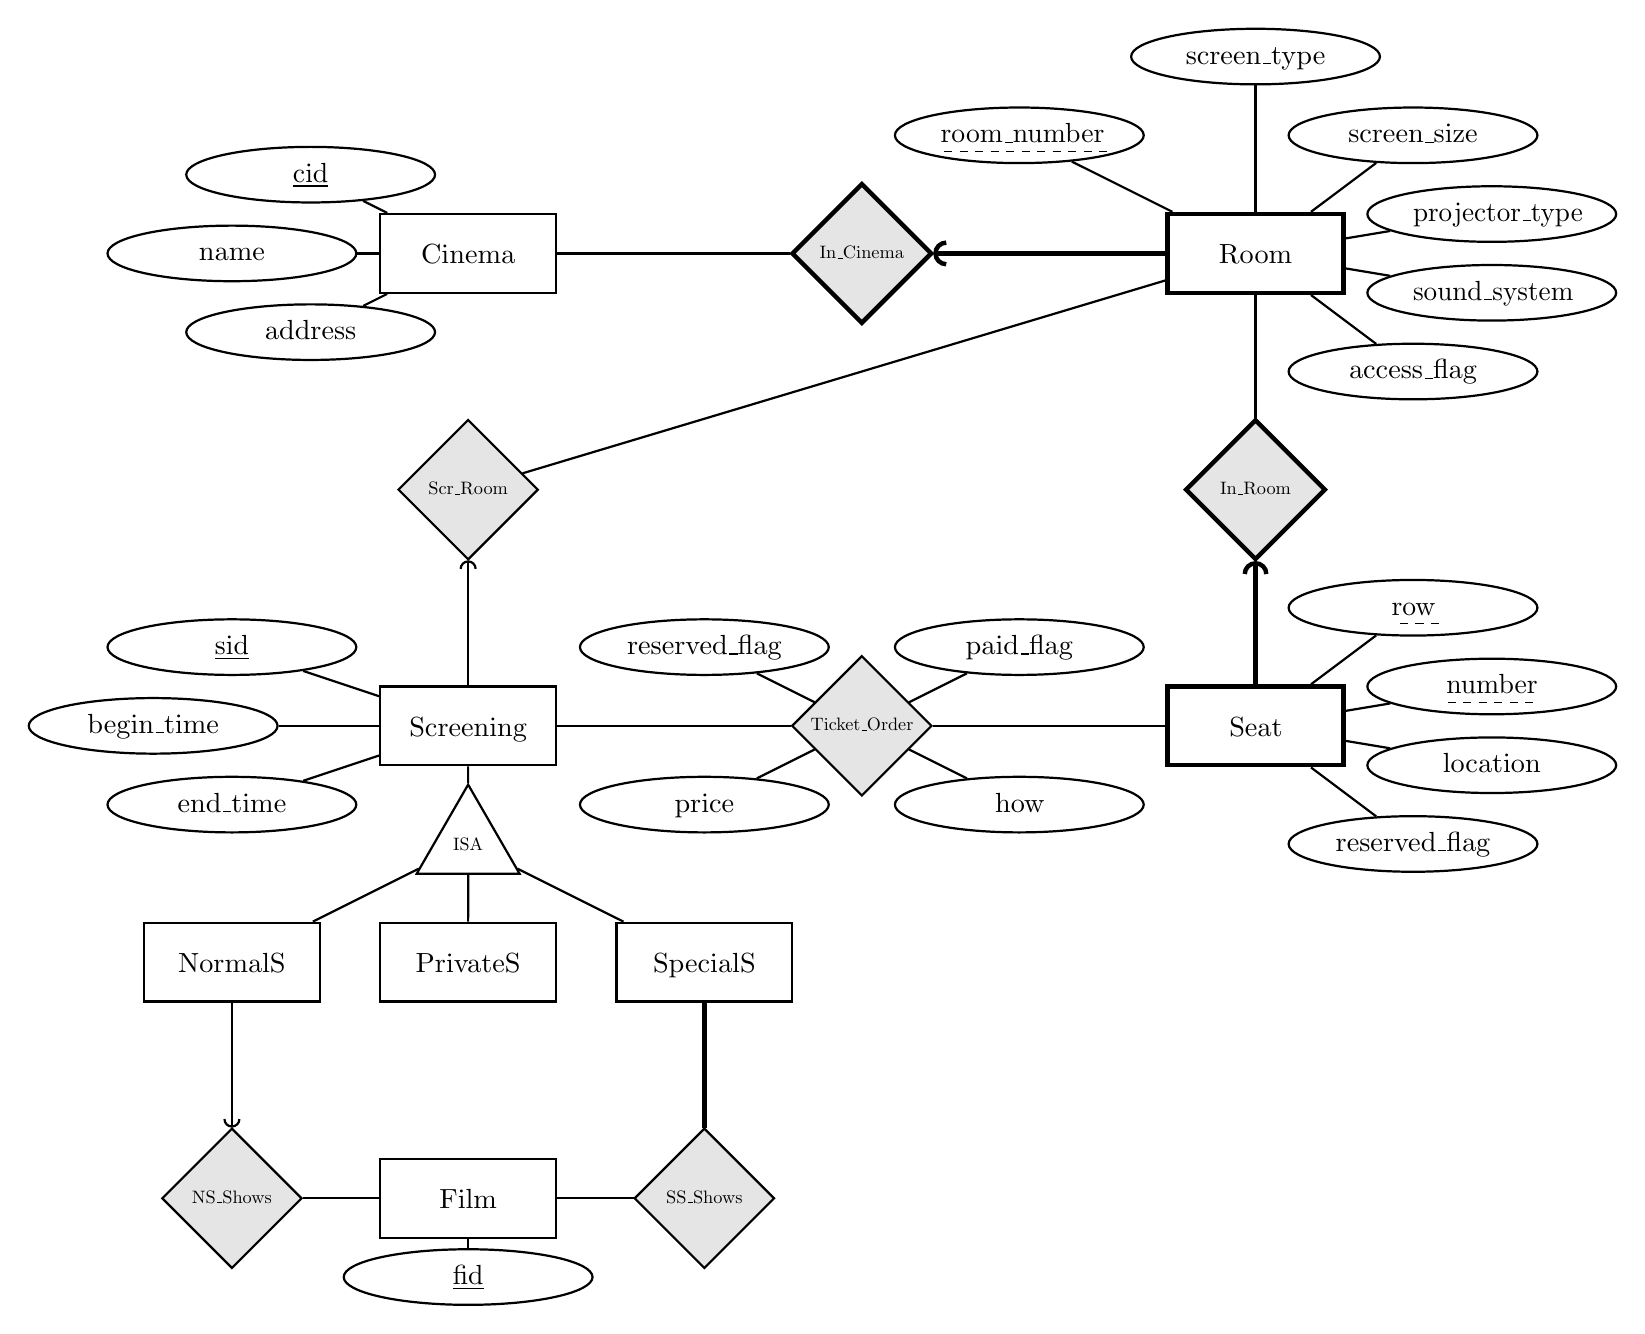
\begin{tikzpicture}[er]
        \node[entity] (c) at (0, 0) {Cinema};
            \node[attr] (cid) at (-2, 1) {\key{cid}} edge (c);
            \node[attr] (cname) at (-3, 0) {name} edge (c);
            \node[attr] (caddr) at (-2, -1) {address} edge (c);
        
        \node[rel,weak] (rc) at (5, 0) {In\_Cinema} edge (c);

        \node[entity,weak] (r) at (10, 0) {Room} edge[strict,weak] (rc);
            \node[attr] (rn) at (7, 1.5) {\pkey{room\_number}} edge (r);
            \node[attr] (rsct) at (10, 2.5) {screen\_type} edge (r);
            \node[attr] (rscs) at (12, 1.5) {screen\_size} edge (r);
            \node[attr] (rpt) at (13, 0.5) {projector\_type} edge (r);
            \node[attr] (rss) at (13, -0.5) {sound\_system} edge (r);
            \node[attr] (rsacc) at (12, -1.5) {access\_flag} edge (r);

        \node[rel,weak] (sr) at (10, -3) {In\_Room} edge (r);

        \node[entity,weak] (s) at (10, -6) {Seat} edge[strict,weak] (sr);
            \node[attr] (srow) at (12, -4.5) {\pkey{row}} edge (s);
            \node[attr] (snum) at (13, -5.5) {\pkey{number}} edge (s);
            \node[attr] (sloc) at (13, -6.5) {location} edge (s);
            \node[attr] (sres) at (12, -7.5) {reserved\_flag} edge (s);
        
        \node[rel] (scrr) at (0, -3) {Scr\_Room} edge (r);
        
        \node[entity] (scr) at (0, -6) {Screening} edge[strict] (scrr);
            \node[attr] (scrid) at (-3, -5) {\key{sid}} edge (scr);
            \node[attr] (scrts) at (-4, -6) {begin\_time} edge (scr);
            \node[attr] (scrts) at (-3, -7) {end\_time} edge (scr);
        \node[isa] (scisa) at (0, -7.5) {} edge (scr);
        
        \node[rel] (nss) at (-3, -12) {NS\_Shows};
        \node[rel] (sss) at (3, -12) {SS\_Shows};

        \node[entity] (f) at (0, -12) {Film} edge (nss) edge (sss);
        \node[attr] (fid) at (0, -13) {\key{fid}} edge (f);
        
        
        \node[entity] (scrn) at (-3, -9) {NormalS} edge (scisa) edge[strict] (nss);
        \node[entity] (scrs) at (3, -9) {SpecialS} edge (scisa) edge[total] (sss);
        \node[entity] (scrp) at (0, -9) {PrivateS} edge (scisa);
        
        \node[rel] (sale) at (5, -6) {Ticket\_Order} edge (scr) edge (s);
            \node[attr] at (3, -5) {reserved\_flag} edge (sale);
            \node[attr] at (7, -5) {paid\_flag} edge (sale);
            \node[attr] at (3, -7) {price} edge (sale);
            \node[attr] at (7, -7) {how} edge (sale);
        
    \end{tikzpicture}
    }
    \caption{The ER-Diagram for the renewed cinema information system.}\label{fig:er}
\end{figure}
\end{document}